\chapter{Overview}
\section{Vitess}\hypertarget{vitess}{}\label{vitess}

Vitess is a set of servers and tools meant to facilitate scaling of MySQL
databases for the web. It's been developed since 2011, and is currently used as
a fundamental component of YouTube's MySQL infrastructure, serving thousands of
QPS (per server). If you want to find out whether Vitess is a good fit for your
project, please read our helicopter overview(~\ref{Helicopter-Overview}).


\section{Overview}\hypertarget{overview}{}\label{overview}

\begin{figure}[H]
\caption{Vitess Overview}
\label{fig:VitessSpectrum}
\begin{center}
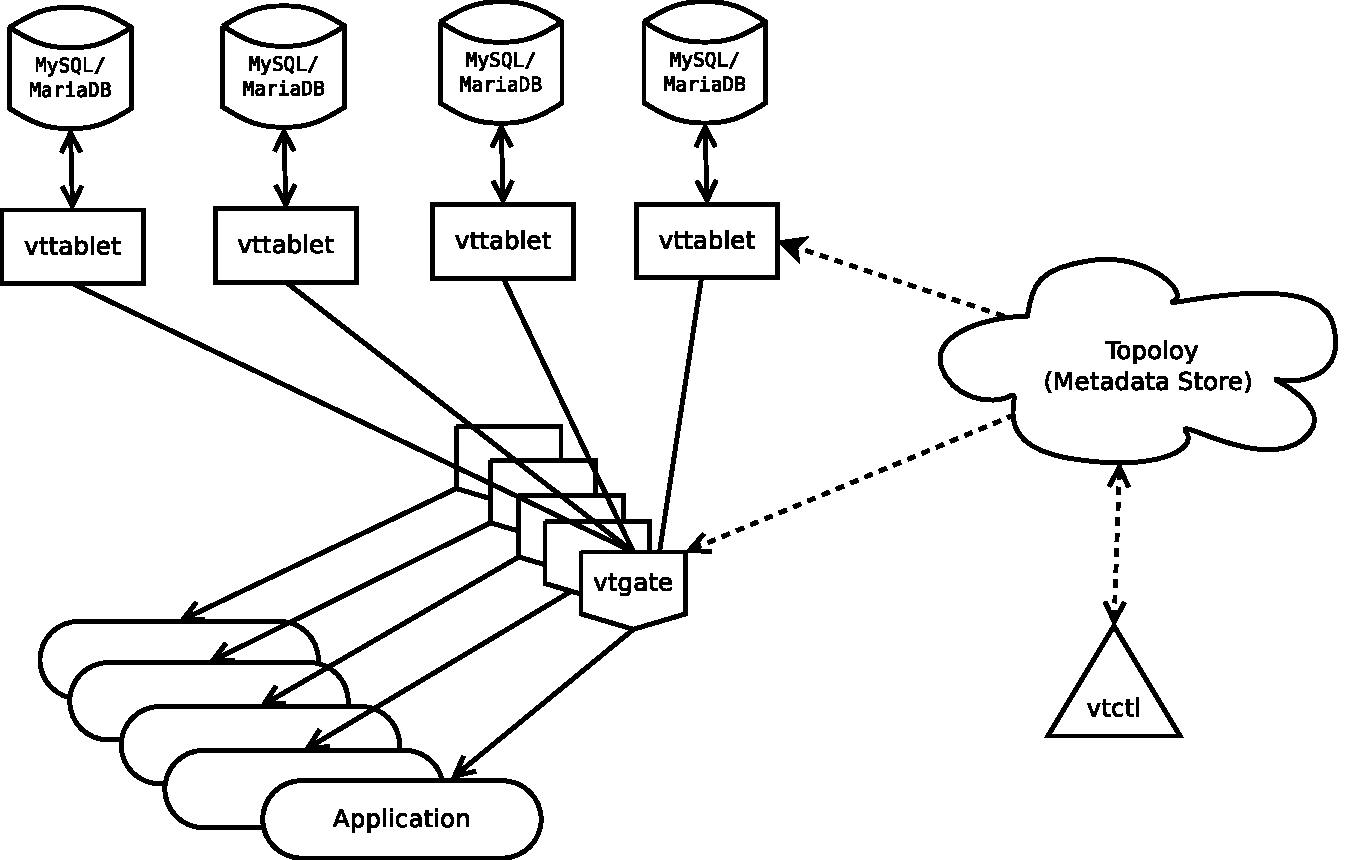
\includegraphics[scale=0.65]{VitessOverview.pdf}
\end{center}
\end{figure}


Vitess consists of a number servers, command line utilities, and a consistent
metadata store. Taken together, they allow you to serve more database traffic,
and add features like sharding, which normally you would have to implement in your
application.

\index{vttable}{\textbf{vttablet}} is a server that sits in front of a MySQL database, making it more
robust and available in the face of high traffic. Among other things, it adds a
connection pool, has a row based cache, and it rewrites SQL queries to be safer
and nicer to the underlying database.


\index{vtgate}{\textbf{vtgate}} is a very light proxy that routes database traffic from your app to the
right vttablet, basing on the sharding scheme, latency required, and health of
the vttablets. This allows the client to be very simple, as all it needs to be
concerned about is finding the closest vtgate.

The \index{topology}{\textbf{topology}} is a metadata store that contains information about running
servers, the sharding scheme, and replication graph. It is backed by a
consistent data store, like \href{http://zookeeper.apache.org/}{Apache ZooKeeper}.
The topology backends are plugin based, allowing you to write your own if
ZooKeeper doesn't fit your needs. You can explore the topology through
\index{vtctld}{\textbf{vtctld}}, a webserver (not shown in the diagram).

\index{vtctl}{\textbf{vtctl}} a command line utility that allows a human or a script to easily
interact with the system.

All components communicate using a lightweight RPC system based on
\href{http://bsonspec.org/}{BSON}. The RPC system is plugin based, so you can easily
write your own backend (at Google we use a Protocol Buffers based protocol). We
provide a client implementation for three languages: Python, Go, and Java.
Writing a client for your language should not be difficult, as it's a matter of
implementing only a few API calls (please send us a pull request if you do!).

To learn more, please click on the documentation links below.
You can also watch a \href{https://www.youtube.com/watch?v=midJ6b1LkA0}{9 minute introduction}
to Vitess \href{https://github.com/sougou}{sougou} prepared for Google I/O 2014.
There's also a longer presentation from the Fosdem `14 go devroom
(\href{https://github.com/youtube/vitess/blob/master/doc/Vitess2014.pdf?raw=true}{slides},
\href{http://youtu.be/qATTTSg6zXk}{video}).

\section{Trying it out}\hypertarget{trying-it-out}{}\label{trying-it-out}

Vitess is not entirely ready for unsupervised use yet. Some functionality is
still under development, APIs may change, and parts of the code are
undocumented. However, if you feel adventurous, you're more than welcome to try
it. We know that there are some rough edges, so please don't hesitate to reach out
to us through \href{https://groups.google.com/forum/\#!forum/vitess}{our mailing list}
if you run into any issues. Warnings aside, please take a look at Getting Started(~\ref{Getting-Started})

guide.

\section{Documentation}\hypertarget{documentation}{}\label{documentation}

\subsection{Intro}\hypertarget{intro}{}\label{intro}

\begin{itemize}
\item Helicopter overview(~\ref{Helicopter-Overview}):  high level overview of Vitess that should tell you whether Vitess is for you.
\item FAQ(~\ref{Vitess-FAQ}):Vitess Frequently Asked Questions.
\item Vision(~\ref{Motivation-and-Vision}): principles guiding the design of Vitess.
\end{itemize}

\subsection{Using Vitess}\label{using-vitess}

\begin{itemize}
\item Getting Started(~\ref{Getting-Started}):  how to set your environment to work with Vitess.
\item Tools and Servers(~\ref{Tools-and-Servers}):  all Vitess tools and servers.
\item Vttablet(~\ref{Vttablet}):  information about the most important Vitess server.
\item Reparenting(~\ref{Reparenting}):  performing master failover.
\item Resharding(~\ref{Resharding}):  adding more shards to your cluster.
\item Preparing for production(~\ref{Production-Setup}): (wip).
\item Schema management(~\ref{Schema-Management}): managing your database schema using Vitess.
\end{itemize}

\subsection{Reference}

\begin{itemize}
\item General Concepts (~\ref{Concepts}):
\item Zookeeper data (~\ref{ZookeeperData}):
\item Serving graph (~\ref{Serving-Graph}):
\item Replication Graph (~\ref{Replication-Graph}):
\end{itemize}

\section{License}\hypertarget{license}{}\label{license}

Unless otherwise noted, the vitess source files are distributed
under the BSD-style license found in the LICENSE file.

